\documentclass[a4paper,12pt]{article}
\usepackage[russian]{babel}

% Самые необходимые пакеты
\usepackage[T2A]{fontenc}
\usepackage[utf8]{inputenc}
\usepackage[russian]{babel}
\usepackage{geometry}
\usepackage{amsmath}
\usepackage{graphicx}
\usepackage{float} 
\usepackage{xcolor}
\usepackage{listings}
\usepackage{hyperref}
\usepackage{array}
\usepackage{caption}
\usepackage{booktabs}
\usepackage{amssymb}
\usepackage{subcaption}
\usepackage{caption}
\captionsetup[figure]{name=Рисунок}
\captionsetup[table]{name=Таблица}
\usepackage{pgfplots}
\pgfplotsset{compat=1.18}
\usetikzlibrary{arrows.meta}
\usepackage{capt-of}
\usepackage{multirow}
\usepackage[siunitx]{circuitikz}
\usepackage[bottom]{footmisc}
\usepackage{tcolorbox}


\lstset{
	language=Matlab,
	basicstyle=\ttfamily\small,
	keywordstyle=\color{blue}\bfseries,
	commentstyle=\color{gray}\itshape,
	stringstyle=\color{red},
	numberstyle=\tiny\color{gray},
	numbers=left,
	stepnumber=1,
	numbersep=8pt,
	backgroundcolor=\color{white},
	frame=single,
	breaklines=true,
	breakatwhitespace=true,
	tabsize=4,
	showspaces=false,
	showstringspaces=false,
	captionpos=b,
	escapeinside={\%*}{*)},
}
\geometry{left=1.5cm, right=2cm, bottom=2cm, top=2cm}

\begin{document}
	
	% Титульный лист
	\begin{titlepage}
		\centering
		
		% Министерство
		\vspace*{0.5cm}
		{\small
			Министерство науки и высшего образования Российской Федерации\\[2pt]
			Федеральное государственное автономное образовательное учреждение\\
			высшего образования\\[2pt]
			\textbf{«Национальный исследовательский университет ИТМО»}\\
		}
		
		\vspace{0.8cm}
		\hrule height 0.8pt
		\vspace{0.3cm}
		
		{\large Факультет систем управления и робототехники}
		
		\vspace{0.3cm}
		\hrule height 0.4pt
		
		\vspace{2.5cm}
		
		% Основной заголовок
		{\Huge\bfseries ОТЧЁТ}\\[0.4cm]
		{\LARGE\bfseries о лабораторной работе}\\[0.8cm]
		
		% Декоративная рамка вокруг темы
		\begin{tcolorbox}[
			colback=gray!4,
			colframe=gray!10,
			boxrule=0.8pt,
			arc=4pt,
			left=12pt, right=12pt, top=8pt, bottom=8pt
			]
			\centering
			{\large По дисциплине:\\[4pt]}
			{\large\bfseries «Теория автоматического управления»}\\[10pt]
			{\large Тема:\\[4pt]}
			{\large\bfseries «Управляемость и наблюдаемость»} \\[10pt]
			{\large Поток: 1.1.3 \( \) Вариант: 25}
		\end{tcolorbox}
		
		\vspace{3cm}
		
		% Студент / Преподаватель
		\begin{minipage}{0.45\textwidth}
			\raggedright
			{\large\bfseries Студент:}\\[4pt]
			Охрименко Е.\,Д.\\
		\end{minipage}
		\hfill
		\begin{minipage}{0.45\textwidth}
			\raggedleft
			{\large\bfseries Преподаватель:}\\[4pt]
			Пашенко А.\,В.\\
		\end{minipage}
		
		\vfill
		
	
		\vspace{0.4cm}
		
		{\large Санкт-Петербург, 2026}
		
	\end{titlepage}
	
	\newpage
	\tableofcontents
	
	
	\newpage
	\section{Исследование управляемости}
	\label{sec:task1}
	В соответствии с моим вариантом рассмотрю систему и точку \(x_1\):
	
	\[
	\dot{x} = A	x + B u 
	\]
	
	\[
	A = 
	\begin{bmatrix}
		5 & -2 & 8 \\
		4 & -3 & 4 \\
		-4 & 0 & -7
	\end{bmatrix}
	\qquad B = 
	\begin{bmatrix}
		-7 \\ -5 \\ 7
	\end{bmatrix}
	\qquad x_1 = 
	\begin{bmatrix}
		-2 \\ -3 \\ 3
	\end{bmatrix}
	\]
	Требуется:
	
	\begin{itemize}
		\item Исследовать управляемость системы тремя методами: найти матрицу 
		управляемости и её ранг, для каждого собственного числа матрицы $A$ 
		построить матрицу Хаутуса и определить её ранг, найти вещественную 
		Жорданову форму системы. По каждому методу сделать вывод об 
		управляемости каждого собственного числа и системы в целом.
		\item Найти Грамиан управляемости $P(t_1)$ при $t_1 = 3$, вычислить 
		его собственные числа и проанализировать их с точки зрения управляемости.
		\item Синтезировать управление $u(t)$, переводящее систему из 
		$x(0) = 0$ в $x(t_1) = x_1$ за время $t_1 = 3$, и выполнить 
		моделирование, подтверждающее корректность расчётов.
	\end{itemize}
	
	\hrule
	
	\newpage	
	\subsection{Матрица управляемости}
	
	Найду матрицу управляемости системы:
	
	\[
	U = 
	\begin{bmatrix}
		B & A B & A^2 B
	\end{bmatrix}
	\]
	
	\[
	AB =
	\begin{bmatrix}
		5 & -2 & 8 \\
		4 & -3 & 4 \\
		-4 & 0 & -7
	\end{bmatrix}
	\begin{bmatrix}-7\\-5\\7\end{bmatrix}
	=
	\begin{bmatrix}
		5\cdot(-7) + (-2)\cdot(-5) + 8\cdot7 \\
		4\cdot(-7) + (-3)\cdot(-5) + 4\cdot7 \\
		(-4)\cdot(-7) + 0\cdot(-5) + (-7)\cdot7
	\end{bmatrix}
	=
	\begin{bmatrix} 31 \\ 15 \\ -21 \end{bmatrix}
	\]
	
	\begin{align*}
		A^2B = A(AB) &=
		\begin{bmatrix}
			5 & -2 & 8 \\
			4 & -3 & 4 \\
			-4 & 0 & -7
		\end{bmatrix}
		\begin{bmatrix}31\\15\\-21\end{bmatrix}
		=
		\begin{bmatrix}
			5\cdot31 + (-2)\cdot15 + 8\cdot(-21) \\
			4\cdot31 + (-3)\cdot15 + 4\cdot(-21) \\
			(-4)\cdot31 + 0\cdot15 + (-7)\cdot(-21)
		\end{bmatrix} \\[8pt]
		&=
		\begin{bmatrix}
			155 - 30 - 168 \\
			124 - 45 - 84 \\
			-124 + 0 + 147
		\end{bmatrix}
		=
		\begin{bmatrix} -43 \\ -5 \\ 23 \end{bmatrix}
	\end{align*}
	
	Тогда матрица \(U\):
	
	\[
	U = 
	\begin{bmatrix}
		-7 & 31 & -43 \\
		-5 & 15 & -5 \\
		7 & -21 & 23 \\
	\end{bmatrix}
	\]
	
	Теперь посчитаю ранг матрицы управляемости. Если ее определитель не равен нулю, то ранг равен размерности матрицы.
	Определитель матрицы управляемости:
	
	\[
	\det(U) =
	\begin{vmatrix}
		-7 & 31 & -43 \\
		-5 & 15 & -5 \\
		7 & -21 & 23
	\end{vmatrix}
	= -2415 - 1085 - 4515 + 4515 + 3565 + 735 = 800 \neq 0
	\]
	
	Значит $\operatorname{rank}(U) = 3$. Следовательно, система является \textit{полностью управляемой}.
	
	\subsection{Анализ собственных чисел матрицы системы}
	
	Найду собственные числа матрицы управляемости:
	
	\[
	\operatorname{det}(A -\lambda I) = 0
	\]
	
	\begin{align*}
		\det(A - \lambda I) &=
		(5-\lambda)(-3-\lambda)(-7-\lambda)
		+ (-2)\cdot4\cdot(-4)
		+ 8\cdot4\cdot0 \\
		&\quad - 8\cdot(-3-\lambda)\cdot(-4)
		- (-2)\cdot4\cdot(-7-\lambda)
		- (5-\lambda)\cdot4\cdot0 \\[6pt]
		&= (5-\lambda)(\lambda^2+10\lambda+21) + 32 - 32(3+\lambda) - 8(7+\lambda) \\[6pt]
		&= (5-\lambda)(\lambda^2+10\lambda+21) + 32 - 96 - 32\lambda - 56 - 8\lambda \\[6pt]
		&= (5-\lambda)(\lambda^2+10\lambda+21) - 120 - 40\lambda \\[6pt]
		&= -\lambda^3 - 5\lambda^2 + 29\lambda + 105 - 120 - 40\lambda \\[6pt]
		&= -\lambda^3 - 5\lambda^2 - 11\lambda - 15 \\[6pt]
		&= -(\lambda^3 + 5\lambda^2 + 11\lambda + 15) = 0
	\end{align*}
	
	Получившиеся собственные числа:
	
	\[\sigma(A) = \{-1 \pm 2i, \ -3\}\]
	
	Для каждого собственного числа найду матрицу Хаутуса, определю ранги матриц при помощи функции \texttt{rank()} в матлаб (Листинг~\ref{lst:haut}).
	
	\begin{itemize}
		\item Собственное число: \(\lambda_1 = -1 + 2i\)
		
		\begin{align*}
			H(\lambda_1) &= \begin{bmatrix} A - \lambda_1 I & B \end{bmatrix} =
			\begin{bmatrix}
				5-(-1+2i) & -2 & 8 & -7 \\
				4 & -3-(-1+2i) & 4 & -5 \\
				-4 & 0 & -7-(-1+2i) & 7
			\end{bmatrix} \\[8pt]
			&=
			\begin{bmatrix}
				6-2i & -2 & 8 & -7 \\
				4 & -2-2i & 4 & -5 \\
				-4 & 0 & -6-2i & 7
			\end{bmatrix} 
		\end{align*}
		
		\(\operatorname{rank}(H(\lambda_1)) = 3\). Ранг матрицы Хаутуса равен размерности матрицы системы~--- собственное число управляемо.
		
		
		\item Собственное число: \(\lambda_1 = -1 -  2i\)
		
		\begin{align*}
			H(\lambda_2) &= \begin{bmatrix} A - \lambda_2 I & B \end{bmatrix} =
			\begin{bmatrix}
				5-(-1-2i) & -2 & 8 & -7 \\
				4 & -3-(-1-2i) & 4 & -5 \\
				-4 & 0 & -7-(-1-2i) & 7
			\end{bmatrix} \\[8pt]
			&=
			\begin{bmatrix}
				6+2i & -2 & 8 & -7 \\
				4 & -2+2i & 4 & -5 \\
				-4 & 0 & -6+2i & 7
			\end{bmatrix}
		\end{align*}
		
		\(\operatorname{rank}(H(\lambda_2)) = 3\). Ранг матрицы Хаутуса равен размерности матрицы системы~--- собственное число управляемо.
		
		\item Собственное число: \(\lambda_1 = -3\) 
		
		\begin{align*}
			H(\lambda_3) &= \begin{bmatrix} A - \lambda_3 I & B \end{bmatrix} =
			\begin{bmatrix}
				5-(-3) & -2 & 8 & -7 \\
				4 & -3-(-3) & 4 & -5 \\
				-4 & 0 & -7-(-3) & 7
			\end{bmatrix} \\[8pt]
			&=
			\begin{bmatrix}
				8 & -2 & 8 & -7 \\
				4 & 0 & 4 & -5 \\
				-4 & 0 & -4 & 7
			\end{bmatrix}
		\end{align*}
		
		\(\operatorname{rank}(H(\lambda_3)) = 3\). Ранг матрицы Хаутуса равен размерности матрицы системы~--- собственное число управляемо.
		
	\end{itemize}
	
	
	Поскольку ранг матрицы Хаутуса равен $n = 3$ для каждого собственного числа матрицы $A$, по критерию Хаутуса система является полностью управляемой.
	
	\subsection{Жорданова форма системы}
	
	Найду собственные векторы матрицы $A$. Собственные векторы для $\lambda_{1,2} = -1 \pm 2i$.
	
	Решу систему $(A - \lambda_1 I)v = 0$:
	\[
	A - \lambda_1 I = 
	\begin{bmatrix}
		6-2i & -2 & 8 \\
		4 & -2-2i & 4 \\
		-4 & 0 & -6-2i
	\end{bmatrix}
	\]
	Собственный вектор для $\lambda_1 = -1 + 2i$:
	\[
	v_1 = \begin{bmatrix} -\dfrac{3}{2} + \dfrac{1}{2}i \\ -1 \\ 1 \end{bmatrix}
	= \underbrace{\begin{bmatrix} -\dfrac{3}{2} \\ -1 \\ 1 \end{bmatrix}}_{\operatorname{Re}(v_1)}
	+ i\underbrace{\begin{bmatrix} \dfrac{1}{2} \\ 0 \\ 0 \end{bmatrix}}_{\operatorname{Im}(v_1)}
	\]
	
	Собственный вектор для $\lambda_3 = -3$. Решу систему $(A - \lambda_3 I)v = 0$:
	\[
	A - \lambda_3 I = 
	\begin{bmatrix}
		8 & -2 & 8 \\
		4 & 0 & 4 \\
		-4 & 0 & -4
	\end{bmatrix}
	\]
	Собственный вектор:
	\[
	v_3 = \begin{bmatrix} -1 \\ 0 \\ 1 \end{bmatrix}
	\]
	
	Матрица перехода строится из вещественной части, мнимой части 
	комплексного вектора и вещественного собственного вектора:
	\[
	P = \begin{bmatrix} \operatorname{Re}(v_1) & \operatorname{Im}(v_1) & v_3 \end{bmatrix}
	= \begin{bmatrix} 
		-\dfrac{3}{2} & \dfrac{1}{2} & -1 \\ 
		-1 & 0 & 0 \\ 
		1 & 0 & 1 
	\end{bmatrix} \qquad
	P^{-1} = \begin{bmatrix} 
		0 & -1 & 0 \\ 
		2 & -1 & 2 \\ 
		0 &  1 & 1 
	\end{bmatrix}
	\]
	
	Тогда вещественная Жорданова форма:
	\begin{align*}
		J_{\mathbb{R}} = P^{-1}AP &= 
		\begin{bmatrix} 0 & -1 & 0 \\ 2 & -1 & 2 \\ 0 & 1 & 1 \end{bmatrix}
		\begin{bmatrix} 5 & -2 & 8 \\ 4 & -3 & 4 \\ -4 & 0 & -7 \end{bmatrix}
		\begin{bmatrix} -\dfrac{3}{2} & \dfrac{1}{2} & -1 \\ -1 & 0 & 0 \\ 1 & 0 & 1 \end{bmatrix} 
		= \begin{bmatrix} -1 & -2 & 0 \\ 2 & -1 & 0 \\ 0 & 0 & -3 \end{bmatrix}
		= \begin{bmatrix} J_1 & \mathbf{0}_{2\times1}  \\
			\mathbf{0}_{1\times2} & J_2  \end{bmatrix}
	\end{align*}
	Жордановы блоки:
	\[
	J_1 = \begin{bmatrix} -1 & -2 \\ 2 & -1 \end{bmatrix} \qquad J_2 = \begin{bmatrix} -3 \end{bmatrix}
	\]
	
	Выполню замену координат $x = P\tilde{x}$. Тогда система 
	$\dot{x} = Ax + Bu$ в Жордановой форме:
	\[
	\dot{\tilde{x}} = J_{\mathbb{R}} \tilde{x} + \tilde{B} u
	\]
	где $\tilde{B} = P^{-1}B$. Найду $\tilde{B}$:
	\[
	\tilde{B} = P^{-1}B = 
	\begin{bmatrix} 0 & -1 & 0 \\ 2 & -1 & 2 \\ 0 & 1 & 1 \end{bmatrix}
	\begin{bmatrix} -7 \\ -5 \\ 7 \end{bmatrix}
	= \begin{bmatrix} 5 \\ 5 \\ 2 \end{bmatrix}
	\]
	
	Тогда система в Жордановой форме:
	\[
	\dot{\tilde{x}} = 
	\begin{bmatrix} -1 & -2 & 0 \\ 2 & -1 & 0 \\ 0 & 0 & -3 \end{bmatrix} \tilde{x} +
	\begin{bmatrix} 5 \\ 5 \\ 2 \end{bmatrix} u
	\]
	
	Блоку $J_1$ (собственные числа $\lambda_{1,2} = -1 \pm 2i$) соответствуют 
	строки 1--2 матрицы $\tilde{B}$: значения $5$ и $5$ --- хотя бы одна из 
	строк ненулевая, собственные числа $\lambda_{1,2}$ управляемы.
	
	Блоку $J_2$ (собственное число $\lambda_3 = -3$) соответствует строка 3: 
	значение $2 \neq 0$, собственное число $\lambda_3$ управляемо.
	
	Таким образом, все собственные числа управляемы, система является 
	полностью управляемой.
	
	\subsection{Грамиан}
	
	Грамиан управляемости вычисляется по формуле:
	\[
	P(t_1) = \int_0^{t_1} e^{At} B B^\top e^{A^\top t}\, dt
	\]
	
	Посчитаю его значение программно (Листинг~\ref{lst:gram}). При $t_1 = 3$ получаю:
	\[
	P(3) = 
	\begin{bmatrix}
		18.1213 & 10.9702 & -11.6368 \\
		10.9702 &  7.4761 &  -8.4761 \\
		-11.6368 & -8.4761 &  10.1428
	\end{bmatrix}
	\]
	
	Собственные числа Грамиана:
	\[
	\mu_1 \approx 33.7426, \qquad \mu_2 \approx 1.9479, \qquad \mu_3 \approx 0.0498
	\]
	
	Все собственные числа Грамиана строго положительны, следовательно матрица $P(t_1)$ является положительно  определённой, что подтверждает полную управляемость системы.
	
	\subsection{Управление}
	
	Найду управление, переводящее систему из $x(0) = 0$ в $x(t_1) = x_1$ 
	за время $t_1 = 3$ по формуле:
	\[
	u(t) = B^\top e^{A^\top(t_1 - t)} \left(P(t_1)\right)^{-1} x_1
	\]
	где $P(t_1)$ --- Грамиан управляемости, вычисленный ранее.
	
	Поскольку система полностью управляема, матрица $P(t_1)$ является 
	положительно определённой и, следовательно обратимой. Подставлю значения:
	\[
	x_1 = \begin{bmatrix} -2 \\ -3 \\ 3 \end{bmatrix}, \qquad
	P(3) = \begin{bmatrix}
		18.1213 & 10.9702 & -11.6368 \\
		10.9702 &  7.4761 &  -8.4761 \\
		-11.6368 & -8.4761 &  10.1428
	\end{bmatrix}
	\]
	
	Управление $u(t)$ вычислю программно (Листинг~\ref{lst:control}).
	
	Нарисую график вектора состояния $x(t)$.
	Пунктирными линиями обозначу целевые значения $x_1 = -2$, $x_2 = -3$, 
	$x_3 = 3$ и момент времени $t_1 = 3$. Видно, что система достигает 
	заданного состояния $x_1$ в момент времени $t_1$.
	
	\begin{figure}[H]
		\centering
		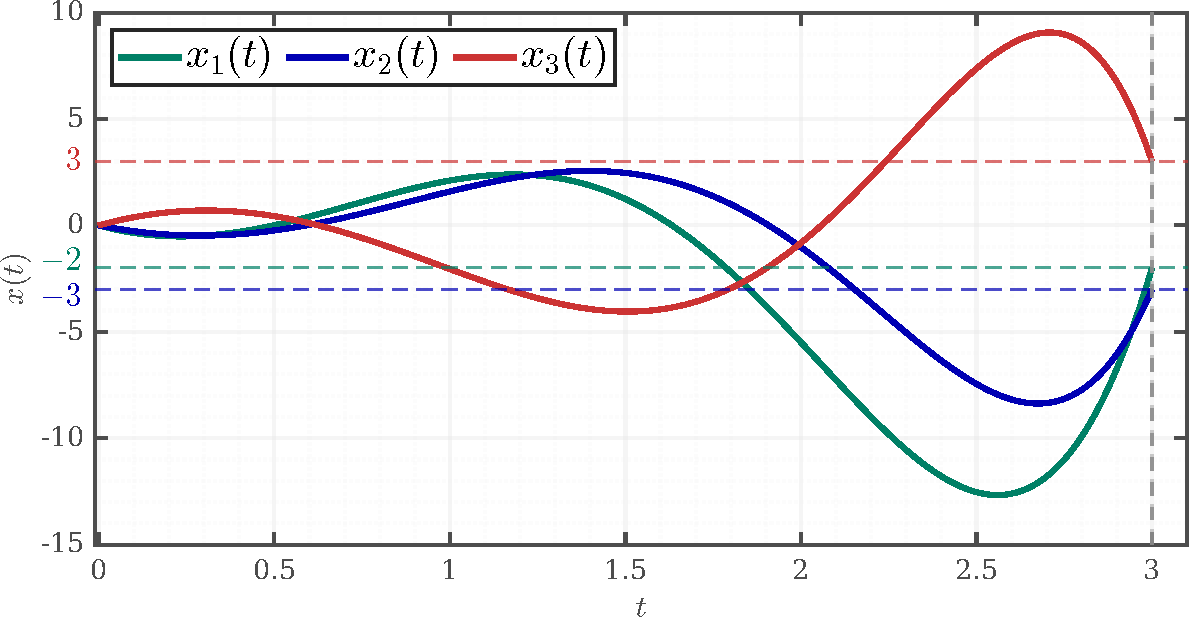
\includegraphics[width=1\textwidth]{../images/task1/x.pdf}
		\caption{Вектор состояния $x(t)$}
	\end{figure}
	
	
	\begin{figure}[H]
		\centering
		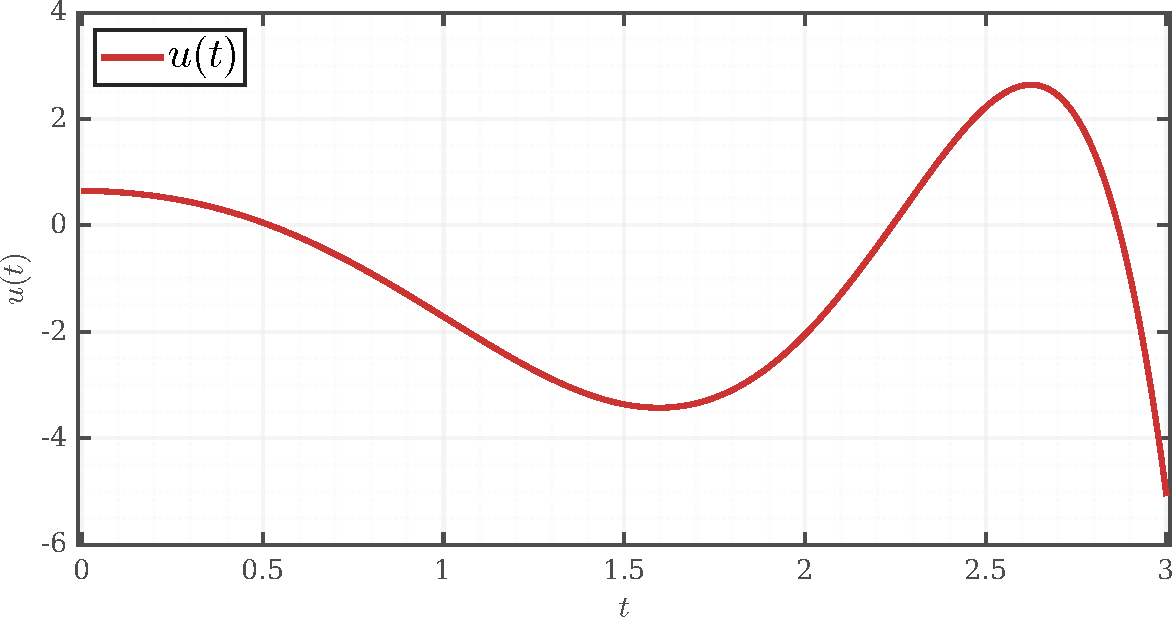
\includegraphics[width=1\textwidth]{../images/task1/u.pdf}
		\caption{Управление $u(t)$}
	\end{figure}
	
	\newpage
	\subsection{Вывод по заданию}
	
	В задании я исследовала управляемость линейной системы $\dot{x} = Ax + Bu$.
	Для этого я использовала три подхода: анализ ранга матрицы управляемости,
	критерий Хаутуса и анализ Жордановой формы. Все три подхода дали одинаковый
	результат --- система является полностью управляемой. Это также подтвердил
	грамиан управляемости $P(t_1)$, все собственные числа которого строго положительные.
	
	Используя Грамиан, я синтезировала программное управление $u(t)$,
	которое переводит систему из нулевого начального состояния $x(0) = 0$
	в заданное состояние $x(t_1) = x_1$ за время $t_1 = 3$.
	Результаты моделирования подтвердили корректность расчётов.
	
	\newpage
	\section{Анализ управляемого подпространства}
	
	В соответствии с вариантом рассмотрю ту же систему, что и в задании 1:
	\[
	\dot{x} = Ax + Bu
	\]
	с матрицей $A$ из задания~1 и новой матрицей $B$:
	\[
	A = \begin{bmatrix}5&-2&8\\4&-3&4\\-4&0&-7\end{bmatrix} \qquad
	B = \begin{bmatrix}-1\\-3\\3\end{bmatrix}
	\]
	Заданы две точки:
	\[
	x'_1 = \begin{bmatrix}-2\\-3\\3\end{bmatrix} \qquad
	x''_1 = \begin{bmatrix}-3\\-3\\4\end{bmatrix}
	\]
	
	Требуется:
	\begin{itemize}
		\item Проверить обе точки $x'_1$ и $x''_1$ на принадлежность 
		управляемому подпространству системы и выбрать ту, что принадлежит.
		\item Для выбранной точки $x_1$ выполнить все шаги задания~1: 
		исследовать управляемость тремя методами, найти Грамиан, 
		синтезировать управление и выполнить моделирование.
	\end{itemize}
	
	\hrule
	
	\newpage
	\subsection{Матрица управляемости}
	
	Найду матрицу управляемости для новой матрицы $B$:
	
	\[
	U = \begin{bmatrix} B & AB & A^2B \end{bmatrix}
	\]
	
	\[
	AB =
	\begin{bmatrix}
		5 & -2 & 8 \\
		4 & -3 & 4 \\
		-4 & 0 & -7
	\end{bmatrix}
	\begin{bmatrix}-1\\-3\\3\end{bmatrix}
	=
	\begin{bmatrix}
		5\cdot(-1) + (-2)\cdot(-3) + 8\cdot3 \\
		4\cdot(-1) + (-3)\cdot(-3) + 4\cdot3 \\
		(-4)\cdot(-1) + 0\cdot(-3) + (-7)\cdot3
	\end{bmatrix}
	=
	\begin{bmatrix} 25 \\ 17 \\ -17 \end{bmatrix}
	\]
	
	\begin{align*}
		A^2B = A(AB) &=
		\begin{bmatrix}
			5 & -2 & 8 \\
			4 & -3 & 4 \\
			-4 & 0 & -7
		\end{bmatrix}
		\begin{bmatrix}25\\17\\-17\end{bmatrix}
		=
		\begin{bmatrix}
			5\cdot25 + (-2)\cdot17 + 8\cdot(-17) \\
			4\cdot25 + (-3)\cdot17 + 4\cdot(-17) \\
			(-4)\cdot25 + 0\cdot17 + (-7)\cdot(-17)
		\end{bmatrix} \\[8pt]
		&=
		\begin{bmatrix}
			125 - 34 - 136 \\
			100 - 51 - 68 \\
			-100 + 0 + 119
		\end{bmatrix}
		=
		\begin{bmatrix} -45 \\ -19 \\ 19 \end{bmatrix}
	\end{align*}
	
	Тогда матрица $U$:
	
	\[
	U = 
	\begin{bmatrix}
		-1 & 25 & -45 \\
		-3 & 17 & -19 \\
		3 & -17 & 19
	\end{bmatrix}
	\]
	
	\subsection{Проверка принадлежности управляемому подпространству}
	
	Точка $x_1$ принадлежит управляемому подпространству системы, если она 
	является линейной комбинацией столбцов матрицы управляемости $U$. 
	Для проверки этого условия сравню ранги:
	\[
	\operatorname{rank}(U) = \operatorname{rank}\begin{bmatrix} U & x_1 \end{bmatrix}
	\]
	Если ранги совпадают, точка принадлежит управляемому подпространству.
	
	Вычислю ранги трех матриц программно (Листинг~\ref{lst:subspace}):
	\[
	\operatorname{rank}(U) = 2
	\]
	
	Для точки $x'_1 = \begin{bmatrix}-2\\-3\\3\end{bmatrix}$:
	\[
	\operatorname{rank}\begin{bmatrix} U & x'_1 \end{bmatrix} = 2 = \operatorname{rank}(U)
	\]
	Точка $x'_1$ принадлежит управляемому подпространству.
	
	Для точки $x''_1 = \begin{bmatrix}-3\\-3\\4\end{bmatrix}$:
	\[
	\operatorname{rank}\begin{bmatrix} U & x''_1 \end{bmatrix} = 3 \neq \operatorname{rank}(U)
	\]
	Точка $x''_1$ не принадлежит управляемому подпространству.
	
	Таким образом, в качестве целевой точки выбираю $x'_1 = \begin{bmatrix}-2\\-3\\3\end{bmatrix} $.	
	
	\subsection{Анализ собственных чисел матрицы системы}
	
	Матрица $A$ совпадает с матрицей из задания~\ref{sec:task1}, поэтому собственные числа 
	те же:
	\[
	\sigma(A) = \{-1 \pm 2i, \ -3\}
	\]
	
	Построю матрицы Хаутуса для каждого собственного числа, определю их ранги (Листинг~\ref{lst:haut2}).
	
	\begin{itemize}
		\item Собственное число: $\lambda_1 = -1 + 2i$
		
		\begin{align*}
			H(\lambda_1) &= \begin{bmatrix} A - \lambda_1 I & B \end{bmatrix} =
			\begin{bmatrix}
				6-2i & -2 & 8 & -1 \\
				4 & -2-2i & 4 & -3 \\
				-4 & 0 & -6-2i & 3
			\end{bmatrix}
		\end{align*}
		
		$\operatorname{rank}(H(\lambda_1)) = 3 = n$. Собственное число $\lambda_1$ управляемо.
		
		\item Собственное число: $\lambda_2 = -1 - 2i$
		
		\begin{align*}
			H(\lambda_2) &= \begin{bmatrix} A - \lambda_2 I & B \end{bmatrix} =
			\begin{bmatrix}
				6+2i & -2 & 8 & -1 \\
				4 & -2+2i & 4 & -3 \\
				-4 & 0 & -6+2i & 3
			\end{bmatrix}
		\end{align*}
		
		$\operatorname{rank}(H(\lambda_2)) = 3 = n$. Собственное число $\lambda_2$ управляемо.
		
		\item Собственное число: $\lambda_3 = -3$
		
		\begin{align*}
			H(\lambda_3) &= \begin{bmatrix} A - \lambda_3 I & B \end{bmatrix} =
			\begin{bmatrix}
				8 & -2 & 8 & -1 \\
				4 & 0 & 4 & -3 \\
				-4 & 0 & -4 & 3
			\end{bmatrix}
		\end{align*}
		
		$\operatorname{rank}(H(\lambda_3)) = 2 < n$. Собственное число $\lambda_3$ \textit{не управляемо}.
	\end{itemize}
	
	Система не является полностью управляемой, так как собственное число $\lambda_3 = -3$ 
	не управляемо.
	
	\subsection{Жорданова форма системы}
	
	Матрица $A$ совпадает с матрицей из задания~\ref{sec:task1}, поэтому 
	собственные векторы, матрица перехода $P$ и вещественная Жорданова форма 
	$J_{\mathbb{R}}$ те же самые.
	
	Найду матрицу $\tilde{B} = P^{-1}B$ для новой матрицы $B$:
	\[
	\tilde{B} = P^{-1}B = 
	\begin{bmatrix} 0 & -1 & 0 \\ 2 & -1 & 2 \\ 0 & 1 & 1 \end{bmatrix}
	\begin{bmatrix} -1 \\ -3 \\ 3 \end{bmatrix}
	= \begin{bmatrix} 3 \\ 7 \\ 0 \end{bmatrix}
	\]
	
	Тогда система в Жордановой форме:
	\[
	\dot{\tilde{x}} = 
	\begin{bmatrix} -1 & -2 & 0 \\ 2 & -1 & 0 \\ 0 & 0 & -3 \end{bmatrix} \tilde{x} +
	\begin{bmatrix} 3 \\ 7 \\ 0 \end{bmatrix} u
	\]
	
	Блоку $J_1$ (собственные числа $\lambda_{1,2} = -1 \pm 2i$) соответствуют 
	строки 1--2 матрицы $\tilde{B}$: значения $3$ и $7$ --- обе строки ненулевые, 
	собственные числа $\lambda_{1,2}$ управляемы.
	
	Блоку $J_2$ (собственное число $\lambda_3 = -3$) соответствует строка 3: 
	значение $0$, собственное число $\lambda_3$ \textit{не управляемо}.
	
	Так как собственное число $\lambda_3 = -3$ не управляемо, система не является полностью управляемой.
	
	\subsection{Грамиан}
	
	Грамиан управляемости вычисляется по формуле:
	\[
	P(t_1) = \int_0^{t_1} e^{At} B B^\top e^{A^\top t}\, dt
	\]
	
	Посчитаю его значение программно (Листинг~\ref{lst:gram2}). При $t_1 = 3$ получаю:
	\[
	P(3) = 
	\begin{bmatrix}
		26.6475 & 13.3715 & -13.3715 \\
		13.3715 &  8.2796 &  -8.2796 \\
		-13.3715 & -8.2796 &   8.2796
	\end{bmatrix}
	\]
	
	Собственные числа Грамиана:
	\[
	\mu_1 \approx 41.1746 \qquad \mu_2 \approx 2.0320 \qquad \mu_3 = 0
	\]
	
	Одно собственное число Грамиана равно нулю, значит матрица $P(t_1)$ 
	не является положительно определённой. Это подтверждает, что система не 
	является полностью управляемой.
	
	\subsection{Управление}
	
	Найду управление, переводящее систему из $x(0) = 0$ в $x(t_1) = x_1$ 
	за время $t_1 = 3$ по формуле:
	\[
	u(t) = B^\top e^{A^\top(t_1 - t)} \left(P(t_1)\right)^+ x_1
	\]
	где $P(t_1)$ --- Грамиан управляемости, $\left(P(t_1)\right)^+$ --- 
	псевдообратная матрица (так как Грамиан вырожден).
	
	Управление $u(t)$ вычислю программно (Листинг~\ref{lst:control2}).
	
	Нарисую графики вектора состояния $x(t)$ и управления $u(t)$. 
	Пунктирными линиями обозначу целевые значения $x_1 = -2$, $x_2 = -3$, 
	$x_3 = 3$ и момент времени $t_1 = 3$. Видно, что система достигает 
	заданного состояния $x_1$ в момент времени $t_1$, несмотря на то что 
	система не является полностью управляемой. Это возможно, так как 
	выбранная точка $x_1$ принадлежит управляемому подпространству.
	
	
	\begin{figure}[H]
		\centering
		
\includegraphics[width=1\textwidth]{../images/task2/x.pdf}
		\caption{Вектор состояния $x(t)$}
	\end{figure}
	
	
	\begin{figure}[H]
		\centering
		
\includegraphics[width=1\textwidth]{../images/task2/u.pdf}
		\caption{Управление $u(t)$}
	\end{figure}
	
	
	
	\newpage
	\subsection{Вывод по заданию}
	
	В задании я исследовала управляемое подпространство системы.
	Система не является полностью управляемой,
	так как ранг матрицы управляемости меньше размерности системы.
	
	По критерию Хаутуса и Жордановой форме
	собственное число $\lambda_3=-3$ неуправляемо.
	Грамиан управляемости подтверждает этот результат.
	
	Выбранная точка принадлежит управляемому подпространству,
	поэтому система достигает заданного состояния.
	Моделирование подтвердило корректность расчётов.
	
	
	
	\newpage
	\newpage
	\section{Исследование наблюдаемости}
	\label{sec:task3}
	
	В соответствии с моим вариантом рассмотрю систему:
	
	\[
	\begin{cases}
		\dot{x} = Ax \\
		y = Cx
	\end{cases}
	\]
	
	\[
	A = 
	\begin{bmatrix}
		-13 & -36 & -8 \\
		6 & 15 & 2 \\
		-2 & -8 & -3
	\end{bmatrix}
	\qquad C = 
	\begin{bmatrix}
		1 & 4 & 1
	\end{bmatrix}
	\qquad f(t) = 1 e^{-t} \cos 4t + 3 e^{-t} \sin 4t 
	\]
	
	Требуется:
	
	\begin{itemize}
		\item Исследовать наблюдаемость системы тремя методами: найти матрицу 
		наблюдаемости и её ранг, для каждого собственного числа матрицы $A$ 
		построить матрицу Хаутуса и определить её ранг, найти вещественную 
		Жорданову форму системы. По каждому методу сделать вывод об 
		наблюдаемости каждого собственного числа и системы в целом.
		\item Найти Грамиан наблюдаемости $Q(t_1)$ при $t_1 = 3$, вычислить 
		его собственные числа и проанализировать их с точки зрения наблюдаемости.
		\item Считая что выход системы $y(t)$ подчиняется закону $y(t) = f(t)$ 
		на временном интервале $t \in [0, t_1]$, определить начальные условия 
		системы и выполнить моделирование, подтверждающее корректность расчётов.
	\end{itemize}
	
	\hrule
	
	\newpage
	\subsection{Матрица наблюдаемости}
	
	Найду матрицу наблюдаемости системы:
	
	\[
	V = 
	\begin{bmatrix}
		C \\ CA \\ CA^2
	\end{bmatrix}
	\]
	Сначала найду соответствующие элементы:	
\[
\begin{aligned}
	CA &=
	\begin{bmatrix}
		1 & 4 & 1
	\end{bmatrix}
	\begin{bmatrix}
		-13 & -36 & -8 \\
		6 & 15 & 2 \\
		-2 & -8 & -3
	\end{bmatrix}
	=
	\begin{bmatrix}
		9 & 16 & -3
	\end{bmatrix}
	\\[6pt]
	CA^2 &=
	\begin{bmatrix}
		9 & 16 & -3
	\end{bmatrix}
	\begin{bmatrix}
		-13 & -36 & -8 \\
		6 & 15 & 2 \\
		-2 & -8 & -3
	\end{bmatrix}
	=
	\begin{bmatrix}
		-15 & -60 & -31
	\end{bmatrix}
\end{aligned}
\]
	Матрица наблюдаемости системы:

	\[
	V = 
	\begin{bmatrix}
		1 & 4 & 1 \\
		9 & 16 & -3 \\
		-15 & -60 & -31
	\end{bmatrix}
	\]
	
	Найду ранг матрицы наблюдаемости в MATLAB (Листинг~\ref{lst:nabl}). Получу:
	
	\[\operatorname{rank}(V) = 3\]
	
	Ранг матрицы наблюдаемости равен размерности системы, значит система полностью наблюдаема.
	
	\subsection{Анализ собственных чисел матрицы системы}
	
	Найду спектр матрицы наблюдаемости:
	
	\[
	\begin{aligned}
		\operatorname{det}(A - \lambda I) &= 0 \\
		\det(A-\lambda I) &=
		\begin{vmatrix}
			-13-\lambda & -36 & -8 \\
			6 & 15-\lambda & 2 \\
			-2 & -8 & -3-\lambda
		\end{vmatrix} =0
	\end{aligned}
	\]
	\[
	\lambda^3 + \lambda^2 + 15\lambda - 17 = 0
	\]
	
	Собственные числа матрицы:
	
	\[
	\sigma(A) = \{-1 \pm 4i, \ 1\}
	\]
	
	Для каждого собственного числа найду матрицу Хаутуса:
	
	\[H(\lambda_i) = \begin{bmatrix} A - \lambda_i I \\ C \end{bmatrix}	\]
	
Вычислю ранги матриц (Листинг~\ref{lst:haut3}), сравню их с размерностью матрицы системы и сделаю выводы о наблюдаемости собственных чисел.

\begin{itemize}
	
	\item Для первого собственного числа $\lambda_1 = -1 + 4i$:
	
	\[
	H(\lambda_1)=
	\begin{bmatrix}
		A-\lambda_1 I \\
		C
	\end{bmatrix}
	=
	\begin{bmatrix}
		-12-4i & -36 & -8 \\
		6 & 16-4i & 2 \\
		-2 & -8 & -2-4i \\
		1 & 4 & 1
	\end{bmatrix}
	\]
	
	Ранг матрицы Хаутуса равен 3, ранг совпадает с размерностью матрицы $A$, следовательно собственное число наблюдаемо.
	
	\item Для второго собственного числа $\lambda_2 = -1 - 4i$:
	
	\[
	\begin{aligned}
		H(\lambda_2) &=
		\begin{bmatrix}
			-13-(-1 - 4i) & -36 & -8 \\
			6 & 15-(-1 - 4i) & 2 \\
			-2 & -8 & -3-(-1 - 4i) \\
			1 & 4 & 1
		\end{bmatrix} \\[8pt]
		&=
		\begin{bmatrix}
			-12 + 4i & -36 & -8 \\
			6 & 16 + 4i & 2 \\
			-2 & -8 & -2 + 4i \\
			1 & 4 & 1
		\end{bmatrix}
	\end{aligned}
	\]
	
	Ранг матрицы Хаутуса равен 3, следовательно собственное число наблюдаемо.
	
	\item Для третьего собственного числа $\lambda_3 = 1$:
	
	\[
	\begin{aligned}
		H(\lambda_3) &=
		\begin{bmatrix}
			-13-1 & -36 & -8 \\
			6 & 15-1 & 2 \\
			-2 & -8 & -3-1 \\
			1 & 4 & 1
		\end{bmatrix} \\[8pt]
		&=
		\begin{bmatrix}
			-14 & -36 & -8 \\
			6 & 14 & 2 \\
			-2 & -8 & -4 \\
			1 & 4 & 1
		\end{bmatrix}
	\end{aligned}
	\]
	
	$\operatorname{rank}(H(\lambda_3)) = 3$, значит собственное число наблюдаемо.
	
\end{itemize}

	Так как ранг матрицы Хаутуса равен рангу системы для всех собственных чисел матрицы  \(A\), система является полностью наблюдаемой по критерию Хаутуса.
	
	
	\subsection{Жорданова форма системы}
	
	Ранее я нашла собственные числа матрицы
	\[
	\sigma(A)=\{-1 \pm 4i, \ 1\}
	\]
	
	Поскольку имеется одна комплексно-сопряжённая пара и одно вещественное собственное число то вещественная жорданова форма будет состоять из одного блока размерности $2\times2$ и одного блока размерности $1\times1$.
	
	Найду собственный вектор для $\lambda_1=-1+4i$ из уравнения:
	\[
	(A-\lambda_1 I)v=0
	\]
	
	Решая систему получаю собственный вектор:
	\[
	v_1=
	\begin{bmatrix}
		3+2i \\
		-1-i \\
		1
	\end{bmatrix}
	=
	\begin{bmatrix}
		3 \\
		-1 \\
		1
	\end{bmatrix}
	+
	i
	\begin{bmatrix}
		2 \\
		-1 \\
		0
	\end{bmatrix}
	\]
	
	Для вещественного собственного числа $\lambda_3=1$ решу уравнение:
	\[
	(A-I)v=0
	\]
	
	Получаю собственный вектор:
	\[
	v_3=
	\begin{bmatrix}
		2 \\
		-1 \\
		1
	\end{bmatrix}
	\]
	
	Матрицу перехода формирую из действительной части комплексного вектора, мнимой части и вещественного собственного вектора:
	
	\[
	P=
	\begin{bmatrix}
		3 & 2 & 2 \\
		-1 & -1 & -1 \\
		1 & 0 & 1
	\end{bmatrix}
	\qquad
	P^{-1} =
	\begin{bmatrix}
		1 & 2 & 0 \\
		0 & -1 & -1 \\
		-1 & -2 & 1
	\end{bmatrix}
	\]
	
	Тогда вещественная Жорданова форма:
	\[
	J_{\mathbb{R}} =P^{-1} A P =
	\begin{bmatrix}
		1 & 2 & 0 \\
		0 & -1 & -1 \\
		-1 & -2 & 1
	\end{bmatrix}
	\begin{bmatrix}
		-13 & -36 & -8 \\
		6 & 15 & 2 \\
		-2 & -8 & -3
	\end{bmatrix}
	\begin{bmatrix}
		3 & 2 & 2 \\
		-1 & -1 & -1 \\
		1 & 0 & 1
	\end{bmatrix}
	=
	\begin{bmatrix}
		-1 & 4 & 0 \\
		-4 & -1 & 0 \\
		0 & 0 & 1
	\end{bmatrix}
	= \begin{bmatrix}
		J_1 & \mathbf{0}_{2\times1}  \\
		\mathbf{0}_{1\times2} & J_2 
	\end{bmatrix}
	\]
	
	Жордановы блоки:
	\[
	J_1 = \begin{bmatrix} -1 & 4 \\ -4 & -1 \end{bmatrix} \qquad J_2 = \begin{bmatrix} 1 \end{bmatrix}
	\]
	
	Выполню замену координат $x = P\tilde{x}$. Тогда система в Жордановой форме имеет вид:
	\[
	\dot{\tilde{x}} = J_{\mathbb{R}}\tilde{x}
	\qquad
	y = \tilde{C}\tilde{x}
	\]
	где $\tilde{C} = CP$. Найду $\tilde{C}$:
	
	\[
	\tilde{C} =
	\begin{bmatrix}
		1 & 4 & 1
	\end{bmatrix}
	\begin{bmatrix}
		3 & 2 & 2 \\
		-1 & -1 & -1 \\
		1 & 0 & 1
	\end{bmatrix}
	=
	\begin{bmatrix}
		0 & -2 & -1
	\end{bmatrix}
	\]
	
	Тогда система в Жордановой форме:
	
	\[
	\dot{\tilde{x}} =
	\begin{bmatrix}
		-1 & 4 & 0 \\
		-4 & -1 & 0 \\
		0 & 0 & 1
	\end{bmatrix}
	\tilde{x}
	\qquad
	y =
	\begin{bmatrix}
		0 & -2 & -1
	\end{bmatrix}
	\tilde{x}
	\]
	
	Блоку $J_1$ (собственные числа $\lambda_{1,2} = -1 \pm 4i$)
	соответствуют координаты $\tilde{x}_1$ и $\tilde{x}_2$.
	Первые два коэффициента матрицы $\tilde{C}$ равны 0 и $-2$.
	Поскольку хотя бы один из них ненулевой, собственные числа $\lambda_{1,2}$ наблюдаемы.
	
	Блоку $J_2$ (собственное число $\lambda_3 = 1$)
	соответствует координата $\tilde{x}_3$.
	Коэффициент равен $-1$ и не равен нулю, следовательно собственное число $\lambda_3$ наблюдаемо.
	
	По итогу все собственные числа наблюдаемы, система является полностью наблюдаемой.
	
	\subsection{Грамиан}
	
	Грамиан наблюдаемости вычисляется по формуле:
	
	\[
	Q(t_1) = \int_0^{t_1} e^{A^\top t} C^\top C \, e^{A t} \, dt
	\]
	
	Вычислю его относительно времени \(t_1 = 3\) (Листинг~\ref{lst:gram_nabl}). Получу:
	
	\[
	\begin{bmatrix}
  202.3098 & 404.5866 & -201.3256 \\
		404.5866 & 810.1626 & -401.3271 \\
		-201.3256 & -401.3271 & 202.8067
	\end{bmatrix}
	\]
	
	Собственные числа Грамиана:
	
	\[
	\mu_1 \approx 1212.0167
	\qquad
	\mu_2 \approx 0.0483421
	\qquad
	\mu_3 \approx 3.2141701
	\]
		
	Поскольку Грамиан наблюдаемости получился положительно определенной матрицей, то система полностью наблюдаема.
	
	\subsection{Начальное условие}
	
	Найду начальное состояние системы $x(0)$ по измеряемому выходу $y(t)$
	на интервале времени $t \in [0,t_1]$.
	
	Начальное состояние определяется по формуле:
	\[
	x(0) =
	\left(Q(t_1)\right)^{-1}
	\int_0^{t_1}
	e^{A^\top t} C^\top y(t) \, dt
	\]
	где $Q(t_1)$ --- Грамиан наблюдаемости.

	Подставляя найденный ранее Грамиан наблюдаемости и закон изменения выхода:
	\[
	y(t) = e^{-t}\cos 4t + 3e^{-t}\sin 4t
	\]
	начальное состояние $x(0)$ вычисляю программно
	(Листинг~\ref{lst:init_state}). Получившийся вектор начальных условий:
	
	\[x(0) = 
	\begin{bmatrix}
		3.5 \\ -1 \\ 1.5
	\end{bmatrix}
	\]
	
	Для проверки корректности найденных начальных условий выполню моделирование. На графике покажу сравнение выхода системы $y(t)$ и заданного сигнала $f(t)$.
	
	
	\begin{figure}[H]
		\centering
		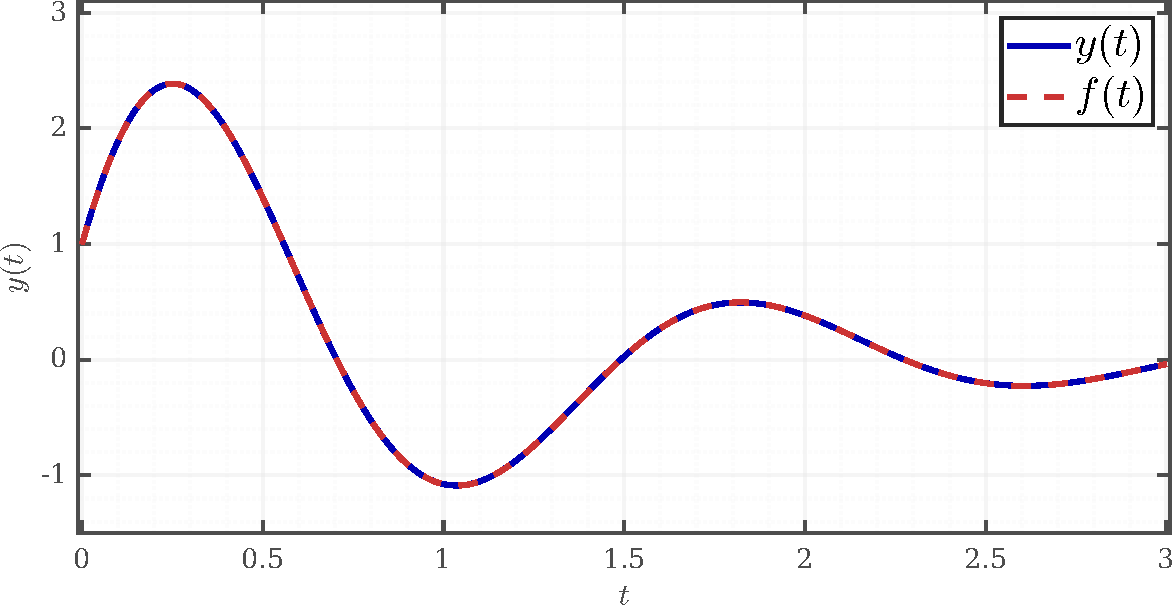
\includegraphics[width=1\textwidth]{../images/task3/uf.pdf}
		\caption{Выход системы $y(t)$ и заданный сигнал $f(t)$}
	\end{figure}
	
	На графике представлю ошибку восстановления:
	\[
	e(t)=y(t)-f(t)
	\]
	Ошибка не превышает $6\cdot10^{-4}$. Погрешность связана с численным вычислением интеграла.
	
	\begin{figure}[H]
		\centering
		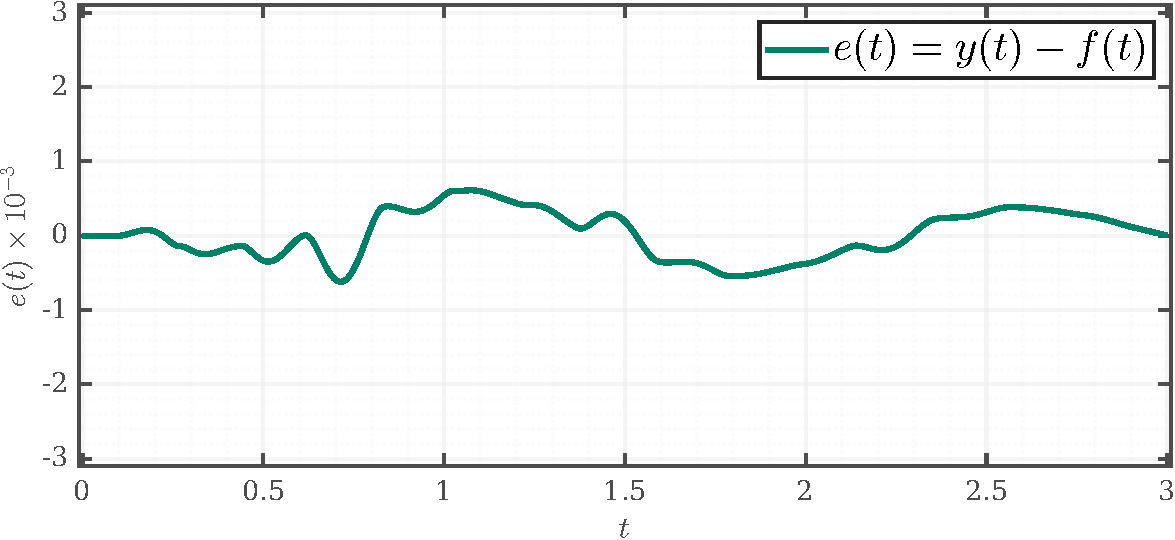
\includegraphics[width=1\textwidth]{../images/task3/e.pdf}
		\caption{Ошибка $e(t)=y(t)-f(t)$}
	\end{figure}
	
	\newpage
	\subsection{Вывод по заданию}
	
	В задании я исследовала наблюдаемость системы.
	Матрица наблюдаемости имеет полный ранг,
	поэтому система полностью наблюдаема.
	
	Критерий Хаутуса, Жорданова форма
	и Грамиан наблюдаемости дали одинаковый результат.
	
	Начальное состояние я нашла по заданному выходу.
	Моделирование подтвердило корректность расчётов.
	
	\newpage
	\section{Анализ ненаблюдаемого подпространства}
	
	В соответствии с вариантом рассмотрю ту же систему, что и в задании~3:
	\[
	\begin{cases}
		\dot{x} = Ax \\
		y = Cx
	\end{cases}
	\]
	с матрицей $A$ из задания~\ref{sec:task3} и новой матрицей $C$:
	\[
	A =
	\begin{bmatrix}
		-13 & -36 & -8 \\
		6 & 15 & 2 \\
		-2 & -8 & -3
	\end{bmatrix}
	\qquad C =
	\begin{bmatrix}
		0 & 4 & 4
	\end{bmatrix}
	\qquad f(t) = e^{-t}\cos 4t + 3e^{-t}\sin 4t
	\]
	
	Требуется:
	
	\begin{itemize}
		\item Исследовать наблюдаемость системы тремя методами (матрица наблюдаемости, критерий Хаутуса, Жорданова форма) и сделать выводы.
		\item Найти Грамиан наблюдаемости $Q(t_1)$ при $t_1 = 3$, проанализировать его собственные числа.
		\item Определить начальные условия по выходу $y(t) = f(t)$ и выполнить моделирование.
		\item Определить, мог ли выход $y(t) = f(t)$ быть порождён иными начальными условиями. Если да~--- привести не менее трёх таких векторов и выполнить моделирование для каждого.
	\end{itemize}
	
	\hrule
	
	\newpage
	\subsection{Матрица наблюдаемости}
	
	Найду матрицу наблюдаемости системы:
	
	\[
	V =
	\begin{bmatrix}
		C \\ CA \\ CA^2
	\end{bmatrix}
	\]
	
	Сначала найду соответствующие элементы:
	\[
	\begin{aligned}
		CA &=
		\begin{bmatrix}
			0 & 4 & 4
		\end{bmatrix}
		\begin{bmatrix}
			-13 & -36 & -8 \\
			6 & 15 & 2 \\
			-2 & -8 & -3
		\end{bmatrix}
		=
		\begin{bmatrix}
			16 & 28 & -4
		\end{bmatrix}
		\\[6pt]
		CA^2 &=
		\begin{bmatrix}
			16 & 28 & -4
		\end{bmatrix}
		\begin{bmatrix}
			-13 & -36 & -8 \\
			6 & 15 & 2 \\
			-2 & -8 & -3
		\end{bmatrix}
		=
		\begin{bmatrix}
			-32 & -124 & -60
		\end{bmatrix}
	\end{aligned}
	\]
	
	Матрица наблюдаемости системы:
	
	\[
	V =
	\begin{bmatrix}
		0 & 4 & 4 \\
		16 & 28 & -4 \\
		-32 & -124 & -60
	\end{bmatrix}
	\]
	
	Найду ранг матрицы наблюдаемости в MATLAB (Листинг~\ref{lst:nabl4}). Получу:
	
	\[\operatorname{rank}(V) = 2 < 3\]
	
	Ранг матрицы наблюдаемости меньше размерности системы, значит система \textit{не является} полностью наблюдаемой.
	
	
	\subsection{Анализ собственных чисел матрицы системы}
	
	Матрица $A$ совпадает с матрицей из задания~\ref{sec:task3}, поэтому собственные числа
	те же:
	\[
	\sigma(A) = \{-1 \pm 4i, \ 1\}
	\]
	
	Построю матрицы Хаутуса для каждого собственного числа, определю их ранги
	(Листинг~\ref{lst:haut4}).
	
	\begin{itemize}
		
		\item Собственное число: $\lambda_1 = -1 + 4i$
		
		\[
		H(\lambda_1) =
		\begin{bmatrix}
			A - \lambda_1 I \\
			C
		\end{bmatrix}
		=
		\begin{bmatrix}
			-12-4i & -36 & -8 \\
			6 & 16-4i & 2 \\
			-2 & -8 & -2-4i \\
			0 & 4 & 4
		\end{bmatrix}
		\]
		
		$\operatorname{rank}(H(\lambda_1)) = 3 = n$. Собственное число $\lambda_1$ наблюдаемо.
		
		\item Собственное число: $\lambda_2 = -1 - 4i$
		
		\[
		H(\lambda_2) =
		\begin{bmatrix}
			A - \lambda_2 I \\
			C
		\end{bmatrix}
		=
		\begin{bmatrix}
			-12+4i & -36 & -8 \\
			6 & 16+4i & 2 \\
			-2 & -8 & -2+4i \\
			0 & 4 & 4
		\end{bmatrix}
		\]
		
		$\operatorname{rank}(H(\lambda_2)) = 3 = n$. Собственное число $\lambda_2$ наблюдаемо.
		
		\item Собственное число: $\lambda_3 = 1$
		
		\[
		H(\lambda_3) =
		\begin{bmatrix}
			A - \lambda_3 I \\
			C
		\end{bmatrix}
		=
		\begin{bmatrix}
			-14 & -36 & -8 \\
			6 & 14 & 2 \\
			-2 & -8 & -4 \\
			0 & 4 & 4
		\end{bmatrix}
		\]
		
		$\operatorname{rank}(H(\lambda_3)) = 2 < n$. Собственное число $\lambda_3$ \textit{не наблюдаемо}.
		
	\end{itemize}
	
	Система не является полностью наблюдаемой, так как собственное число $\lambda_3 = 1$
	не наблюдаемо.
	
	
	\subsection{Жорданова форма системы}
	
	Матрица $A$ совпадает с матрицей из задания~\ref{sec:task3}, поэтому
	собственные векторы, матрица перехода $P$ и вещественная Жорданова форма
	$J_{\mathbb{R}}$ те же самые:
	
	\[
	P=
	\begin{bmatrix}
		3 & 2 & 2 \\
		-1 & -1 & -1 \\
		1 & 0 & 1
	\end{bmatrix}
	\qquad
	J_{\mathbb{R}} =
	\begin{bmatrix}
		-1 & 4 & 0 \\
		-4 & -1 & 0 \\
		0 & 0 & 1
	\end{bmatrix}
	\]
	
	Найду матрицу $\tilde{C} = CP$ для новой матрицы $C$:
	
	\[
	\tilde{C} =
	\begin{bmatrix}
		0 & 4 & 4
	\end{bmatrix}
	\begin{bmatrix}
		3 & 2 & 2 \\
		-1 & -1 & -1 \\
		1 & 0 & 1
	\end{bmatrix}
	=
	\begin{bmatrix}
		0 & -4 & 0
	\end{bmatrix}
	\]
	
	Тогда система в Жордановой форме:
	
	\[
	\dot{\tilde{x}} =
	\begin{bmatrix}
		-1 & 4 & 0 \\
		-4 & -1 & 0 \\
		0 & 0 & 1
	\end{bmatrix}
	\tilde{x}
	\qquad
	y =
	\begin{bmatrix}
		0 & -4 & 0
	\end{bmatrix}
	\tilde{x}
	\]
	
	Блоку $J_1$ (собственные числа $\lambda_{1,2} = -1 \pm 4i$)
	соответствуют координаты $\tilde{x}_1$ и $\tilde{x}_2$.
	Первые два коэффициента матрицы $\tilde{C}$ равны $0$ и $-4$.
	Поскольку хотя бы один из них ненулевой, собственные числа $\lambda_{1,2}$ наблюдаемы.
	
	Блоку $J_2$ (собственное число $\lambda_3 = 1$)
	соответствует координата $\tilde{x}_3$.
	Коэффициент равен $0$, следовательно собственное число $\lambda_3$ \textit{не наблюдаемо}.
	
	Таким образом, система не является полностью наблюдаемой.
	
	\subsection{Грамиан}
	
	Грамиан наблюдаемости вычисляется по формуле:
	
	\[
	Q(t_1) = \int_0^{t_1} e^{A^\top t} C^\top C \, e^{A t} \, dt
	\]
	
	Вычислю его относительно времени $t_1 = 3$ (Листинг~\ref{lst:gram4}). Получу:
	
	\[
	Q(3) =
	\begin{bmatrix}
		3.7572 & 8.4550 & 0.9407 \\
		8.4550 & 23.0145 & 6.1044 \\
		0.9407 & 6.1044 & 4.2230
	\end{bmatrix}
	\]
	
	Собственные числа Грамиана:
	
	\[
	\mu_1 \approx 27.7561 \qquad \mu_2 \approx 3.2385 \qquad \mu_3 = 0
	\]
	
	Одно собственное число Грамиана равно нулю, следовательно матрица $Q(t_1)$
	не является положительно определённой. Это подтверждает, что система не
	является полностью наблюдаемой.
	
	
	\subsection{Начальное условие}
	
	Найду начальное состояние системы $x(0)$ по измеряемому выходу $y(t)$
	на интервале времени $t \in [0, t_1]$.
	
	Начальное состояние определяется по формуле:
	\[
	x(0) = \left(Q(t_1)\right)^{+} \int_0^{t_1} e^{A^\top t} C^\top y(t) \, dt
	\]
	где $Q(t_1)$ --- Грамиан наблюдаемости, $\left(Q(t_1)\right)^{+}$ ---
	псевдообратная матрица (так как Грамиан вырожден).
	
	Подставляя найденный ранее Грамиан наблюдаемости и закон изменения выхода:
	\[
	y(t) = e^{-t}\cos 4t + 3e^{-t}\sin 4t
	\]
	начальное состояние $x(0)$ вычисляю программно
	(Листинг~\ref{lst:init_state4}). Получившийся вектор начальных условий:
	
	\[
	x(0) =
	\begin{bmatrix}
		0.1667 \\ 0.2917 \\ -0.0417
	\end{bmatrix}
	\]
	
	На графике покажу сравнение выхода системы $y(t)$ и заданного сигнала $f(t)$.
	
	
	\begin{figure}[H]
		\centering
		
\includegraphics[width=1\textwidth]{../images/task4/uf.pdf}
		\caption{Выход системы $y(t)$ и заданный сигнал $f(t)$}
	\end{figure}
	
	На графике представлю ошибку восстановления:
	\[
	e(t)=y(t)-f(t)
	\]
	Ошибка не превышает $4\cdot10^{-3}$. Погрешность связана с численным вычислением интеграла.
	
	\begin{figure}[H]
		\centering
		
\includegraphics[width=1\textwidth]{../images/task4/e.pdf}
		\caption{Ошибка $e(t)=y(t)-f(t)$}
	\end{figure}	
	
	\subsection{Альтернативные начальные условия}
	
	Ранее я показала, что система не является полностью наблюдаемой. Это означает, что один и тот же выход \(y(t)\) может быть порожден различными начальными состояниями.
	
	Ненаблюдаемое подпространство представляет собой ядро матрицы наблюдаемости \(V\). Нужно решить однородную систему \(V v = 0\):
	\[
	\begin{bmatrix}
		0 & 4 & 4 \\
		16 & 28 & -4 \\
		-32 & -124 & -60
	\end{bmatrix} v = 0
	\qquad \Longrightarrow \qquad
	\begin{cases}
		4v_2 + 4v_3 = 0 \\
		16v_1 + 28v_2 - 4v_3 = 0 \\
		-32v_1 - 124v_2 - 60v_3 = 0
	\end{cases}
	\]
	После преобразований, получаю, что все векторы ненаблюдаемого подпространства имеют вид:
	\[
	v = v_3 \cdot \begin{bmatrix} 2 \\ -1 \\ 1 \end{bmatrix}
	\]
	Базисный вектор ненаблюдаемого подпространства:
	\[
	\vec{e} = \begin{bmatrix} 2 \\ -1 \\ 1 \end{bmatrix}
	\]
	
	Любой вектор начальных условий \(\tilde{x}(0)\), дающий тот же выход \(y(t) = f(t)\), что и найденный ранее \(x(0)\), может быть представлен как сумма исходного вектора и вектора из ненаблюдаемого подпространства:
	\[
	\tilde{x}(0) = x(0) + \alpha \cdot \vec{e} \qquad \alpha \in \mathbb{R}
	\]
	Для демонстрации корректности выполненных расчетов выберу три различных значения параметра \(\alpha\):
	\begin{itemize}
		\item \(\alpha = 0\):
		\[
		x_1(0) = \begin{bmatrix} 0.1667 \\ 0.2917 \\ -0.0417 \end{bmatrix}
		\]
		\item \(\alpha = 1\):
		\[
		x_2(0) = \begin{bmatrix} 0.1667 \\ 0.2917 \\ -0.0417 \end{bmatrix} + \begin{bmatrix} 2 \\ -1 \\ 1 \end{bmatrix} = \begin{bmatrix} 2.1667 \\ -0.7083 \\ 0.9583 \end{bmatrix}
		\]
		\item \(\alpha = -1\):
		\[
		x_3(0) = \begin{bmatrix} 0.1667 \\ 0.2917 \\ -0.0417 \end{bmatrix} - \begin{bmatrix} 2 \\ -1 \\ 1 \end{bmatrix} = \begin{bmatrix} -1.8333 \\ 1.2917 \\ -1.0417 \end{bmatrix}
		\]
	\end{itemize}
	
	На рисунках ниже представлю траектории компонент вектора состояния $x(t)$ при различных начальных условиях.
	
		
	\begin{figure}[H]
		\centering
		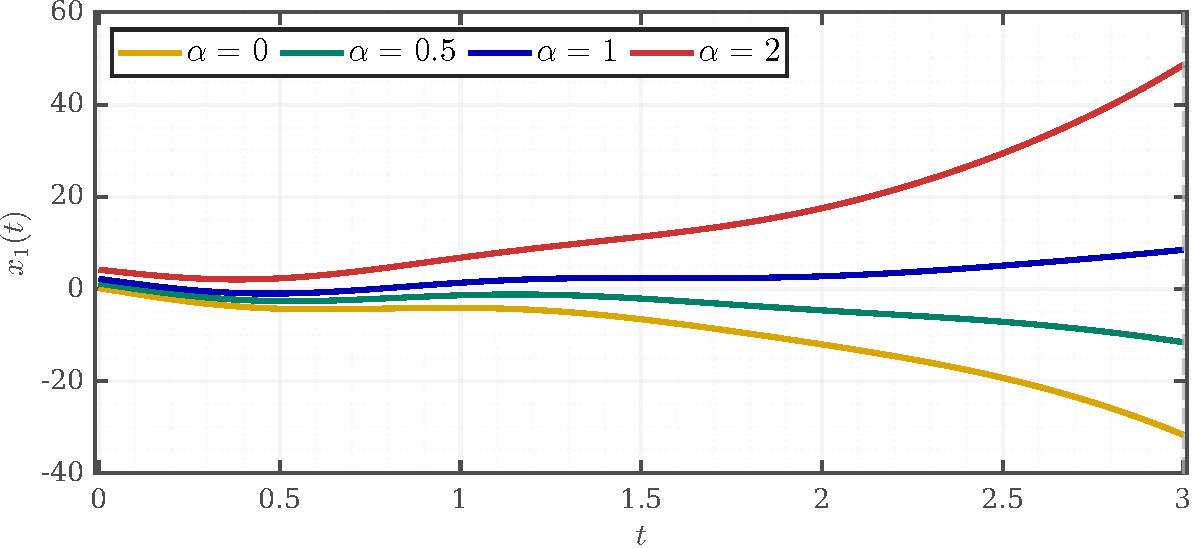
\includegraphics[width=1\textwidth]{../images/task4/x1.pdf}
		\caption{Компонента $x_1(t)$ при различных начальных условиях}
	\end{figure}
	
	
		\begin{figure}[H]
		\centering
		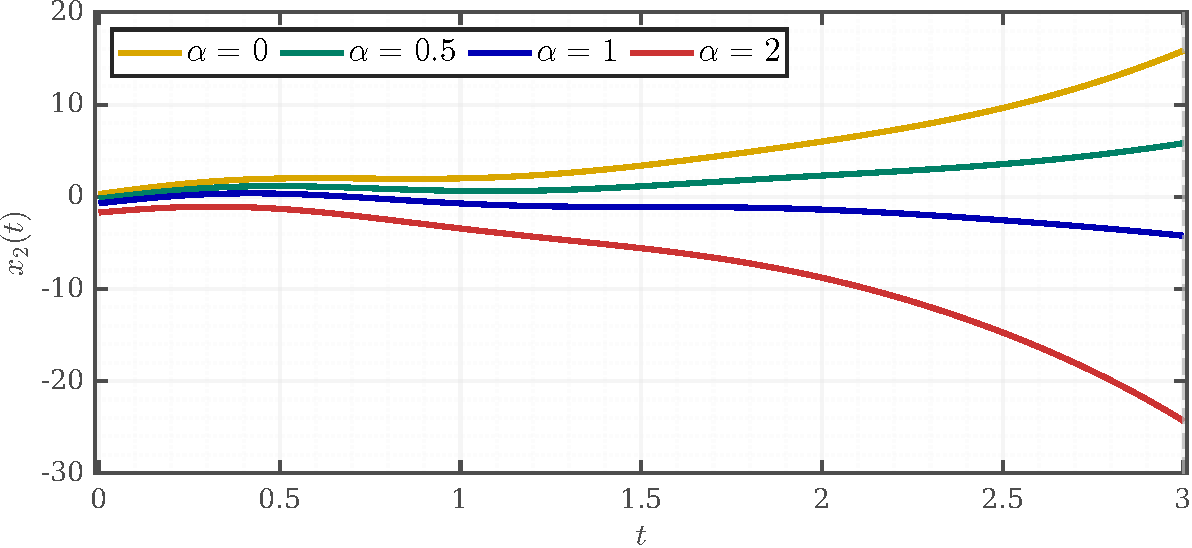
\includegraphics[width=1\textwidth]{../images/task4/x2.pdf}
		\caption{Компонента $x_2(t)$ при различных начальных условиях}
	\end{figure}
	
	
	\begin{figure}[H]
		\centering
		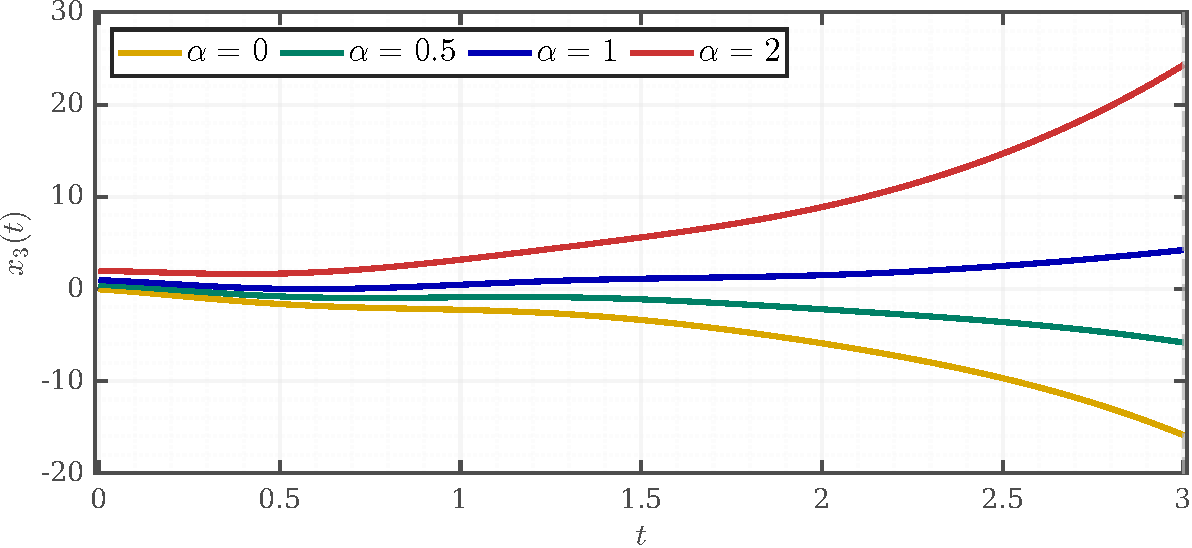
\includegraphics[width=1\textwidth]{../images/task4/x3.pdf}
		\caption{Компонента $x_3(t)$ при различных начальных условиях}
	\end{figure}
	
	
	Как видно из графиков, траектории компонент различаются 
	в зависимости от выбранного $\alpha$, но все они стартуют из 
	различных начальных условий, что хорошо видно при $t = 0$.
	
	Для более наглядного отображения начальных условий приведу 
	приближение графиков в окрестности $t = 0$.
	
	\begin{figure}[H]
		\centering
		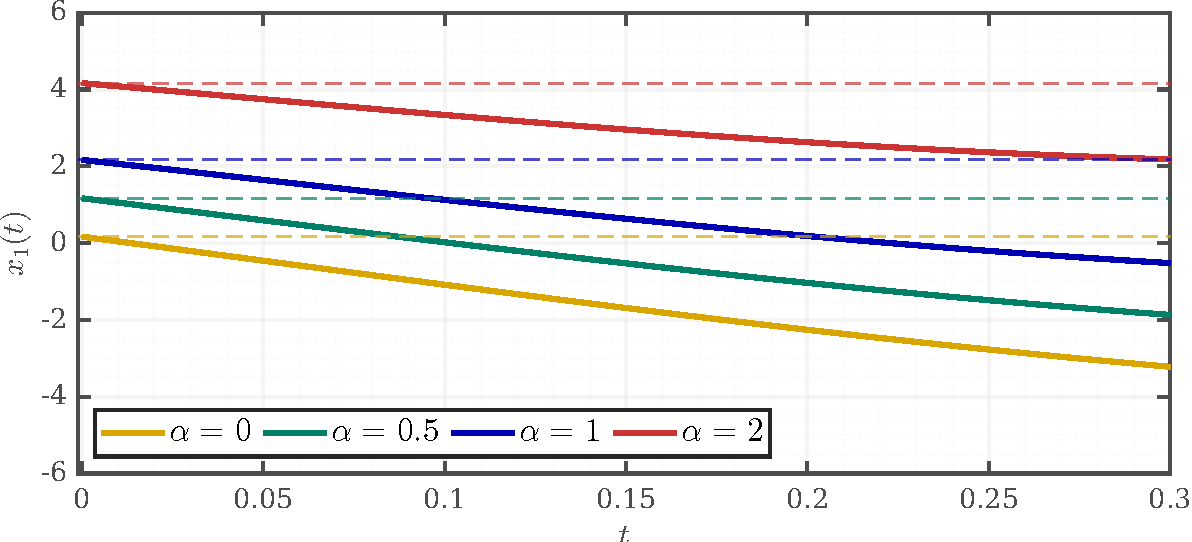
\includegraphics[width=1\textwidth]{../images/task4/x1_zoom.pdf}
		\caption{Приближенная компонента $x_1(t)$ при различных начальных условиях}
	\end{figure}
	
	
	\begin{figure}[H]
		\centering
		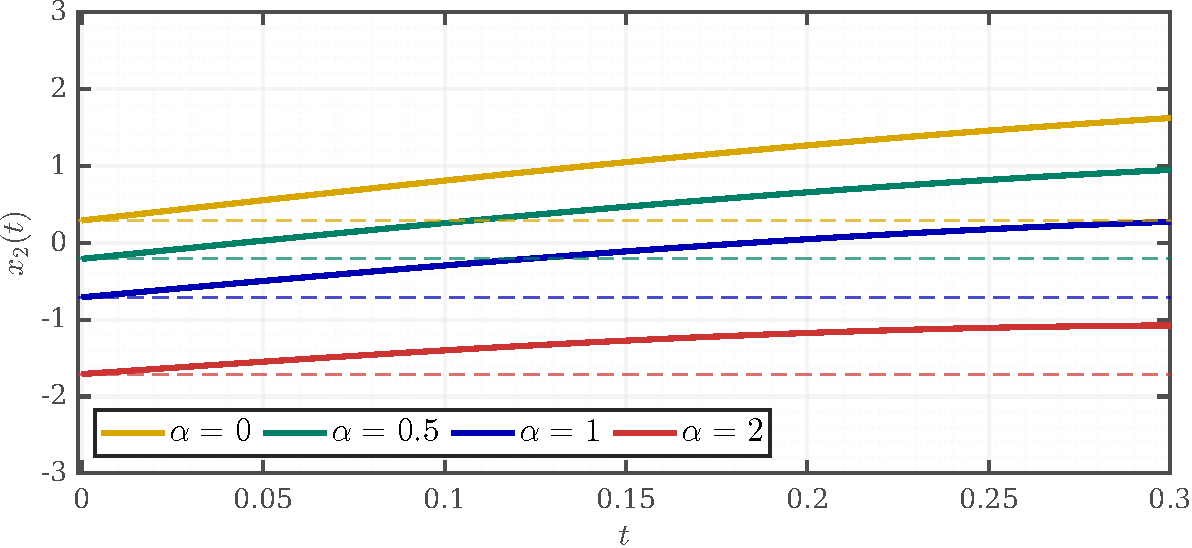
\includegraphics[width=1\textwidth]{../images/task4/x2_zoom.pdf}
		\caption{Приближенная компонента $x_2(t)$ при различных начальных условиях}
	\end{figure}
	
	
	\begin{figure}[H]
		\centering
		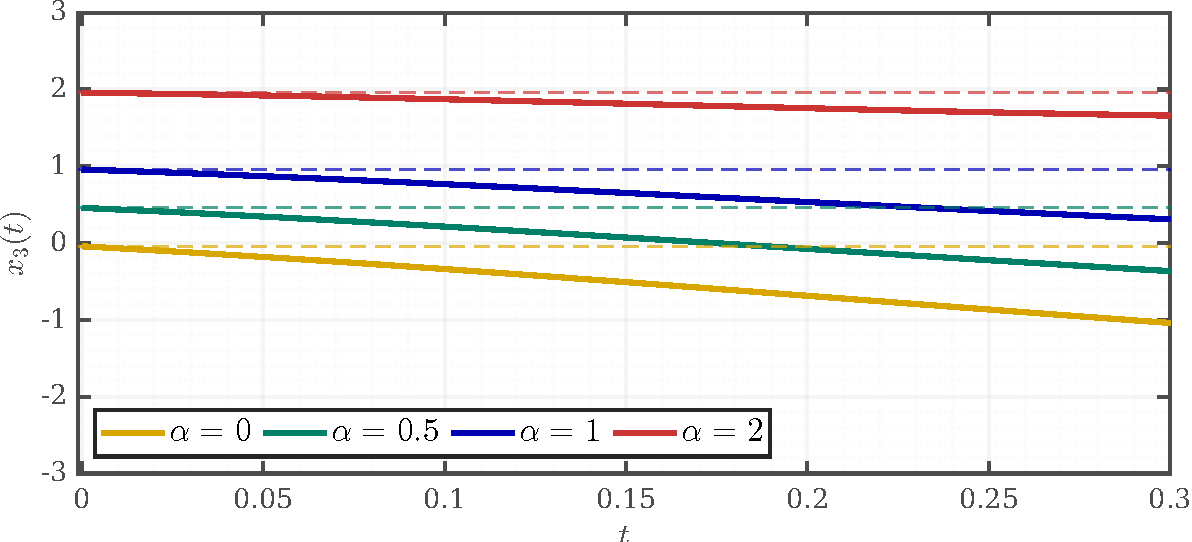
\includegraphics[width=1\textwidth]{../images/task4/x3_zoom.pdf}
		\caption{Приближенная компонента $x_3(t)$ при различных начальных условиях}
	\end{figure}
	
	На графике ниже представлены выходы системы $y(t)$ при всех четырёх 
	начальных условиях на одной координатной плоскости. Несмотря на 
	существенно различающиеся траектории состояний, выход системы 
	остаётся одинаковым для всех $\alpha$ --- это это означает, 
	что добавка $\alpha \cdot \vec{e}$ принадлежит ненаблюдаемому 
	подпространству и не влияет на выход.
	
	\begin{figure}[H]
		\centering
		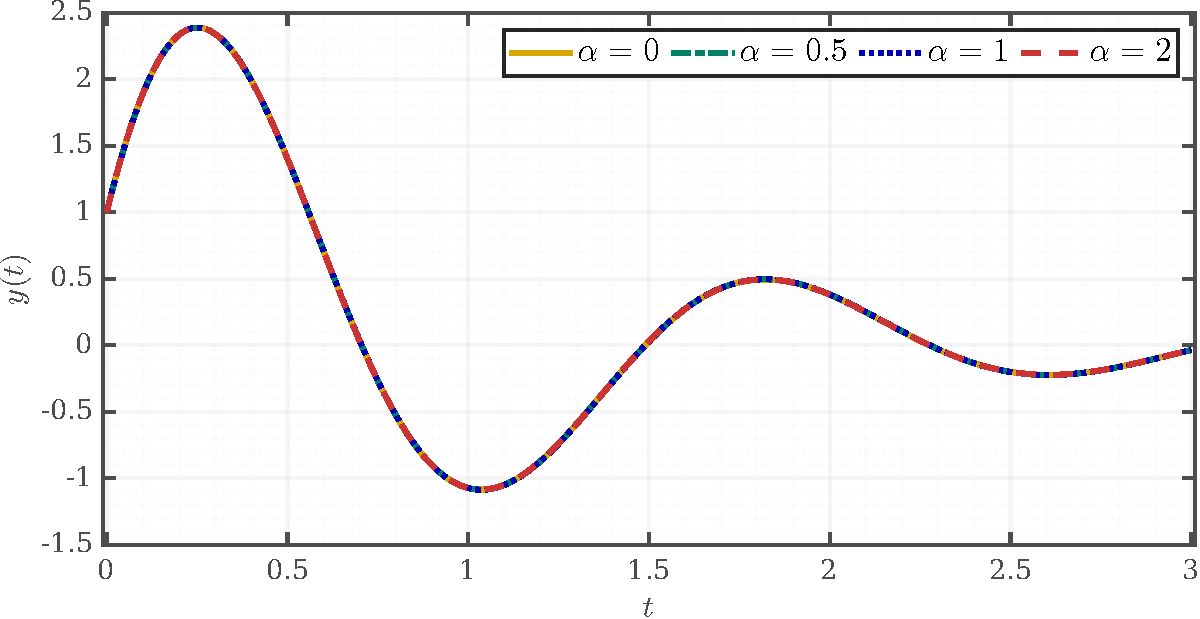
\includegraphics[width=1\textwidth]{../images/task4/y.pdf}
		\caption{Выходы системы $y(t)$ при различных начальных условиях}
	\end{figure}

	\newpage	
	\subsection{Вывод по заданию}
	
	В задании я исследовала ненаблюдаемое подпространство системы.
	Система не является полностью наблюдаемой --- собственное число
	$\lambda_3 = 1$ не наблюдаемо, Грамиан вырожден.
	
	Поскольку система неполностью наблюдаема, один и тот же выход
	$y(t) = f(t)$ может быть порождён бесконечным множеством начальных
	условий вида $\tilde{x}(0) = x(0) + \alpha\cdot\vec{e}$.
	Моделирование подтвердило корректность расчётов.
	
	
	\newpage
	\section{Исследование управляемости по выходу}
	
	В соответствии с вариантом рассмотрю систему:
	
	\[
	\begin{cases}
		\dot{x} = Ax + Bu \\
		y = Cx + Du
	\end{cases}
	\]
	
	с матрицей $A$ из задания~\ref{sec:task1} и матрицами $B$ и $C$:
	
	\[
	A =
	\begin{bmatrix}
		5 & -2 & 8 \\
		4 & -3 & 4 \\
		-4 & 0 & -7
	\end{bmatrix}
	\qquad
	B =
	\begin{bmatrix}
		-1 \\ -3 \\ 3
	\end{bmatrix}
	\qquad
	C =
	\begin{bmatrix}
		0 & 3 & 5 \\
		0 & 14 & 9
	\end{bmatrix}
	\qquad
	D = \mathbf{0}_{2\times 1}
	\]
	
	Требуется:
	
	\begin{itemize}
		\item Найти вещественную Жорданову форму системы.
		\item Определить управляемость и наблюдаемость каждого из 
		собственных чисел и системы в целом.
		\item Найти матрицу управляемости системы по выходу при 
		$D = \mathbf{0}_{2\times1}$, определить её ранг и сделать вывод 
		об управляемости по выходу.
		\item Проанализировать зависимость управляемости по выходу от 
		(не)управляемости и (не)на-
		блюдаемости собственных чисел.
		\item Если система не полностью управляема по выходу~--- предложить 
		матрицу $D$, обеспечивающую полную управляемость по выходу.
	\end{itemize}
	
	\hrule
	
\newpage
\subsection{Жорданова форма системы}

Исходная система в жордановой форме принимает вид:
\[
\dot{\tilde{x}} = J_R \tilde{x} + \tilde{B}u
\]

Ранее я нашла:

\[
P =
\begin{bmatrix}
	-\dfrac{3}{2} & \dfrac{1}{2} & -1 \\
	-1 & 0 & 0 \\
	1 & 0 & 1
\end{bmatrix}
\qquad
P^{-1} =
\begin{bmatrix}
	0 & -1 & 0 \\
	2 & -1 & 2 \\
	0 & 1 & 1
\end{bmatrix}
\qquad
J_R = P^{-1}AP =
\begin{bmatrix}
	-1 & -2 & 0 \\
	2 & -1 & 0 \\
	0 & 0 & -3
\end{bmatrix}
\]

Жорданова форма состоит из двух блоков:
\[
J_R =
\begin{bmatrix}
	J_1 & 0_{2\times1} \\
	0_{1\times2} & J_2
\end{bmatrix}
\qquad
J_1 =
\begin{bmatrix}
	-1 & -2 \\
	2 & -1
\end{bmatrix}
\qquad
J_2 = [-3]
\]

Матрица входа в новых координатах:
\[
\tilde{B} = P^{-1}B =
\begin{bmatrix}
	0 & -1 & 0 \\
	2 & -1 & 2 \\
	0 & 1 & 1
\end{bmatrix}
\begin{bmatrix}
	-1 \\ -3 \\ 3
\end{bmatrix}
=
\begin{bmatrix}
	3 \\
	7 \\
	0
\end{bmatrix}
\]


Матрица выхода в новых координатах определяется как:
\[
\tilde{C} = CP
\]

Подставляя матрицы $C$ и $P$, получаю:
\[
\tilde{C} =
\begin{bmatrix}
	0 & 3 & 5 \\
	0 & 14 & 9
\end{bmatrix}
\begin{bmatrix}
	-\dfrac{3}{2} & \dfrac{1}{2} & -1 \\
	-1 & 0 & 0 \\
	1 & 0 & 1
\end{bmatrix}
=
\begin{bmatrix}
	2 & 0 & 5 \\
	-5 & 0 & 9
\end{bmatrix}
\]

Тогда система в жордановых координатах принимает вид:
\[
\begin{aligned}
	\begin{cases}
		\dot{\tilde{x}} =
		\begin{bmatrix}
			-1 & -2 & 0 \\
			2 & -1 & 0 \\
			0 & 0 & -3
		\end{bmatrix}
		\tilde{x}
		+
		\begin{bmatrix}
			3 \\
			7 \\
			0
		\end{bmatrix}u \\[25pt]
		y =
		\begin{bmatrix}
			2 & 0 & 5 \\
			-5 & 0 & 9
		\end{bmatrix}
		\tilde{x}
		+ Du
	\end{cases}
\end{aligned}
\]

	
	\subsection{Управляемость и наблюдаемость собственных чисел}
	
	
	Первые две строки матрицы $\tilde{B}$ соответствуют жорданову блоку
	$J_1$, то есть комплексно-сопряжённой паре собственных чисел
	$\lambda_{1,2}=-1\pm2i$. Поскольку хотя бы одна из строк ненулевая,
	получаю:
	\[
	\lambda_{1,2}=-1\pm2i \;\; \text{--- управляемы}
	\]
	
	Третья строка соответствует блоку $J_2$ и собственному числу
	$\lambda_3=-3$. Так как соответствующий элемент равен нулю,
	\[
	\lambda_3=-3 \;\; \text{--- неуправляемо}
	\]
	
	Следовательно, система не является полностью управляемой. \\
	\par		
	Для определения наблюдаемости воспользуюсь жордановым разложением системы.

	
	Блоку $J_1$ (собственные числа $\lambda_{1,2}=-1\pm2i$)
	соответствуют первые два столбца матрицы $\tilde{C}$:
	\[
	\begin{bmatrix}
		2 & 0\\
		-5 & 0
	\end{bmatrix}
	\]
	Поскольку хотя бы один элемент ненулевой, $\lambda_{1,2}$ наблюдаемы.
	
	Блоку $J_2$ (собственное число $\lambda_3=-3$)
	соответствует третий столбец:
	\[
	\begin{bmatrix}
		5\\
		9
	\end{bmatrix} \neq 0
	\]
	следовательно $\lambda_3$ наблюдаемо.
	
	Таким образом, все собственные числа наблюдаемы, система является полностью наблюдаемой.
	
	\subsection{Матрица управляемости по выходу}
	Определю матрицу управляемости по выходу и ее ранг для моей системы третьего порядка (Листинг~\ref{lst:555}):
	
	\[
	W_y =
	\begin{bmatrix}
		CB & CAB & CA^2B
	\end{bmatrix}
	\]
	
	\[
	U_y =
	\begin{bmatrix}
		6 & -34 & 38 \\
		-15 & 85 & -95
	\end{bmatrix}
	\qquad
	\operatorname{rank}(U_y)=1
	\]
	
	Поскольку ранг матрицы управляемости по выходу меньше числа выходов системы,
	система не является полностью управляемой по выходу.
	
	\subsection{Анализ и выбор матрицы $D$}
	
	При $D = \mathbf{0}_{2\times1}$ матрица управляемости по выходу:
	\[
	U_y = \begin{bmatrix}6 & -34 & 38\\-15 & 85 & -95\end{bmatrix} \qquad \text{rank}(U_y) = 1 < 2
	\]
	Строки матрицы линейно зависимы, так как каждый столбец пропорционален
	вектору $\begin{bmatrix}2\\-5\end{bmatrix}$:
	\[
	CB = \begin{bmatrix}6\\-15\end{bmatrix} = 3\begin{bmatrix}2\\-5\end{bmatrix} \qquad
	CAB = \begin{bmatrix}-34\\85\end{bmatrix} = -17\begin{bmatrix}2\\-5\end{bmatrix} \qquad
	CA^2B = \begin{bmatrix}38\\-95\end{bmatrix} = 19\begin{bmatrix}2\\-5\end{bmatrix}
	\]
	
	Значит выберу матрицу $D$, не коллинеарную вектору пропорциональности
	строк матрицы управляемости. Например:
	\[
	D = \begin{bmatrix}1\\0\end{bmatrix} \not\parallel \begin{bmatrix}2\\-5\end{bmatrix}
	\]
	Тогда расширенная матрица управляемости по выходу
	$U_y^{\text{ext}} = \begin{bmatrix} D & CB & CAB & CA^2B \end{bmatrix}$:
	\[
	U_y^{\text{ext}} = \begin{bmatrix}1 & 6 & -34 & 38\\0 & -15 & 85 & -95\end{bmatrix}
	\qquad \text{rank}\!\left(U_y^{\text{ext}}\right) = 2
	\]
	Ранг совпадает с числом выходов, значит система стала управляемой по выходу.
	Проверка этого факта находится в Листинге~\ref{lst:UD}.
	
	\newpage
	\subsection{Вывод по заданию}
	
	В задании я исследовала управляемость системы по выходу.
	Собственные числа $\lambda_{1,2} = -1 \pm 2i$ управляемы и наблюдаемы,
	$\lambda_3 = -3$ — наблюдаемо, но неуправляемо.
	
	При $D = \mathbf{0}_{2\times1}$ матрица $U_y$ имеет $\text{rank}(U_y) = 1 < 2$
	— система не является полностью управляемой по выходу. Это следствие
	неуправляемости $\lambda_3 = -3$: режим виден на выходе, но недоступен
	для управления, что приводит к линейной зависимости строк $U_y$.
	
	Введение матрицы $D = \begin{bmatrix}1\\0\end{bmatrix}$ уничтожает линейную
	зависимость, $\text{rank}(U_y^{\text{ext}}) = 2$, система становится
	полностью управляемой по выходу.\\
	
	Закономерность: если собственное
	число одновременно неуправляемо и наблюдаемо, то оно вносит вклад
	в выход, но недоступно для управления — это нарушает управляемость по выходу.
	
	\newpage
	\section{Вывод}
	
	В работе я исследовала управляемость и наблюдаемость линейных систем.
	Неуправляемые собственные числа ограничивают управляемое подпространство,
	а ненаблюдаемые делают восстановление начального состояния неоднозначным.
	При исследовании управляемости по выходу неуправляемое, но наблюдаемое
	собственное число нарушает её; введение матрицы~$D$ устраняет эту проблему.
	
	Материалы работы: \href{https://github.com/decadeos/ITMO/tree/master/3_course/TAU/lab1}{\texttt{github.com}}
	
	\newpage
	\section{Приложение}

\subsection*{Задание 1}

\begin{lstlisting}[caption={Инициализация}]
A = [5 -2 8; 
 4 -3 4; 
	-4 0 -7];

B = [-7; -5; 7]; 
x1 = [-2; -3; 3];

t1 = 3;
\end{lstlisting}

	
\begin{lstlisting}[caption={Вычисление рангов матриц Хаутуса}, label={lst:haut}]
lambda1 = -1 + 2i; lambda2 = -1 - 2i; lambda3 = -3;
rank([A - lambda1*eye(3), B])
rank([A - lambda2*eye(3), B])
rank([A - lambda3*eye(3), B])
\end{lstlisting}
	
\begin{lstlisting}[caption={Грамиан управляемости}, label={lst:gram}]
P = integral(@(t) expm(A*t)*B*B'*expm(A'*t), 0, t1,'ArrayValued', true)
ev = eig(P)
\end{lstlisting}
	
\begin{lstlisting}[caption={Синтез управления}, label={lst:control}]
u = @(t) B' * expm(A'*(t1-t)) * inv(P) * x1;
[t, x] = ode45(@(t,x) A*x + B*u(t), [0 t1], zeros(3,1));
\end{lstlisting}

\newpage
\subsection*{Задание 2}

\begin{lstlisting}[caption={Инициализация}]
A = [5 -2 8; 
 4 -3 4; 
	-4 0 -7];

B = [-1; -3; 3];
x1_p = [-2; -3; 3];
x1_pp = [-3; -3; 4];

t1 = 3;
\end{lstlisting}

\begin{lstlisting}[caption={Вычисление рангов для определения принадлежности к подпространству}, label={lst:subspace}]
U = ctrb(A, B);
r = rank(U)
r_p = rank([U, x1_p])
r_pp = rank([U, x1_pp])
\end{lstlisting}

\begin{lstlisting}[caption={Вычисление рангов матриц Хаутуса}, label={lst:haut2}]
lambda1 = -1 + 2i; lambda2 = -1 - 2i; lambda3 = -3;
rank([A - lambda1*eye(3), B])
rank([A - lambda2*eye(3), B])
rank([A - lambda3*eye(3), B])
\end{lstlisting}

\begin{lstlisting}[caption={Грамиан управляемости}, label={lst:gram2}]
P = integral(@(t) expm(A*t)*B*B'*expm(A'*t), 0, t1, 'ArrayValued', true);
ev = eig(P)
\end{lstlisting}

\begin{lstlisting}[caption={Синтез управления}, label={lst:control2}]
u = @(t) B' * expm(A'*(t1-t)) * pinv(P) * x1;
opts = odeset('MaxStep', 0.01);
[t, x] = ode45(@(t,x) A*x + B*u(t), [0 t1], zeros(3,1), opts);
\end{lstlisting}

\newpage
\subsection*{Задание 3}

\begin{lstlisting}[caption={Инициализация}]
A = [-13 -36 -8;
	  6  15  2;
	 -2  -8 -3];

C = [1 4 1];

f = @(t) exp(-t).*cos(4*t) + 3*exp(-t).*sin(4*t);
t1 = 3
\end{lstlisting}

\begin{lstlisting}[caption={Вычисление ранга матрицы наблюдаемости}, label={lst:nabl}]
O = obsv(A,C)
rank(O)
\end{lstlisting}

\begin{lstlisting}[caption={Вычисление рангов матриц Хаутуса}, label={lst:haut3}]
lambda1 = -1 + 4i; lambda2 = -1 - 4i; lambda3 = 1;
rank([A - lambda1*eye(3); C])
rank([A - lambda2*eye(3); C])
rank([A - lambda3*eye(3); C])
\end{lstlisting}

\begin{lstlisting}[caption={Грамиан наблюдаемости}, label={lst:gram_nabl}]
Q = integral(@(t) expm(A'*t)*C'*C*expm(A*t), 0, t1, 'ArrayValued', true)
ev = eig(Q)
\end{lstlisting}

\begin{lstlisting}[caption={Вычисление начальных условий}, label={lst:init_state}]
I = integral(@(t) expm(A'*t)*C'*f(t), 0, t1, 'ArrayValued', true);
x0 = inv(Q)*I
\end{lstlisting}

\newpage
\subsection*{Задание 4}

\begin{lstlisting}[caption={Инициализация}]
A = [-13 -36 -8;
      6  15  2;
	  -2  -8 -3];
	
C = [0 4 4];
f = @(t) exp(-t).*cos(4*t) + 3*exp(-t).*sin(4*t);
t1 = 3
\end{lstlisting}

\begin{lstlisting}[caption={Вычисление ранга матрицы наблюдаемости}, label={lst:nabl4}]
O = obsv(A,C)
rank(O)
\end{lstlisting}

\begin{lstlisting}[caption={Вычисление рангов матриц Хаутуса}, label={lst:haut4}]
lambda1 = -1 + 4i; lambda2 = -1 - 4i; lambda3 = 1;
rank([A - lambda1*eye(3); C])
rank([A - lambda2*eye(3); C])
rank([A - lambda3*eye(3); C])
\end{lstlisting}

\begin{lstlisting}[caption={Грамиан управляемости}, label={lst:gram4}]
Q = integral(@(t) expm(A'*t)*C'*C*expm(A*t), 0, t1, 'ArrayValued', true)
ev = eig(Q)
\end{lstlisting}

\begin{lstlisting}[caption={Вычисление начальных условий}, label={lst:init_state4}]
I = integral(@(t) expm(A'*t)*C'*f(t), 0, t1, 'ArrayValued', true);
x0 = pinv(Q) * I;
\end{lstlisting}

\newpage
\subsection*{Задание 5}

\begin{lstlisting}[caption={Инициализация}]
A = [5 -2 8;
	 4 -3 4;
	-4 0 -7];
B = [-1; -3; 3];
C = [0 3 5; 0 14 9];
\end{lstlisting}

\begin{lstlisting}[caption={Ранг матрицы управляемости по выходу}, label={lst:555}]
U = [C*B, C*A*B, C*A^2*B]
r = rank(U)
\end{lstlisting}

\begin{lstlisting}[caption={Проверка матрицы управляемости}, label={lst:UD}]
D = [1; 0];
Uy_ext = [D, C*B, C*A*B, C*A^2*B];
rank(Uy_ext)  
\end{lstlisting}

	
\end{document}